\documentclass[journal,12pt,twocolumn]{IEEEtran}

\usepackage{setspace}
\usepackage{gensymb}
\singlespacing
\usepackage[cmex10]{amsmath}

\usepackage{amsthm}

\usepackage{mathrsfs}
\usepackage{txfonts}
\usepackage{stfloats}
\usepackage{bm}
\usepackage{cite}
\usepackage{cases}
\usepackage{subfig}

\usepackage{longtable}
\usepackage{multirow}

\usepackage{enumitem}
\usepackage{mathtools}
\usepackage{steinmetz}
\usepackage{tikz}
\usepackage{circuitikz}
\usepackage{verbatim}
\usepackage{tfrupee}
\usepackage[breaklinks=true]{hyperref}
\usepackage{graphicx}
\usepackage{tkz-euclide}

\usetikzlibrary{calc,math}
\usepackage{listings}
    \usepackage{color}                                            %%
    \usepackage{array}                                            %%
    \usepackage{longtable}                                        %%
    \usepackage{calc}                                             %%
    \usepackage{multirow}                                         %%
    \usepackage{hhline}                                           %%
    \usepackage{ifthen}                                           %%
    \usepackage{lscape}     
\usepackage{multicol}
\usepackage{chngcntr}

\DeclareMathOperator*{\Res}{Res}

\renewcommand\thesection{\arabic{section}}
\renewcommand\thesubsection{\thesection.\arabic{subsection}}
\renewcommand\thesubsubsection{\thesubsection.\arabic{subsubsection}}

\renewcommand\thesectiondis{\arabic{section}}
\renewcommand\thesubsectiondis{\thesectiondis.\arabic{subsection}}
\renewcommand\thesubsubsectiondis{\thesubsectiondis.\arabic{subsubsection}}


\hyphenation{op-tical net-works semi-conduc-tor}
\def\inputGnumericTable{}                                 %%

\lstset{
%language=C,
frame=single, 
breaklines=true,
columns=fullflexible
}
\begin{document}

\newcommand{\BEQA}{\begin{eqnarray}}
\newcommand{\EEQA}{\end{eqnarray}}
\newcommand{\define}{\stackrel{\triangle}{=}}
\bibliographystyle{IEEEtran}
\raggedbottom
\setlength{\parindent}{0pt}
\providecommand{\mbf}{\mathbf}
\providecommand{\pr}[1]{\ensuremath{\Pr\left(#1\right)}}
\providecommand{\qfunc}[1]{\ensuremath{Q\left(#1\right)}}
\providecommand{\sbrak}[1]{\ensuremath{{}\left[#1\right]}}
\providecommand{\lsbrak}[1]{\ensuremath{{}\left[#1\right.}}
\providecommand{\rsbrak}[1]{\ensuremath{{}\left.#1\right]}}
\providecommand{\brak}[1]{\ensuremath{\left(#1\right)}}
\providecommand{\lbrak}[1]{\ensuremath{\left(#1\right.}}
\providecommand{\rbrak}[1]{\ensuremath{\left.#1\right)}}
\providecommand{\cbrak}[1]{\ensuremath{\left\{#1\right\}}}
\providecommand{\lcbrak}[1]{\ensuremath{\left\{#1\right.}}
\providecommand{\rcbrak}[1]{\ensuremath{\left.#1\right\}}}
\theoremstyle{remark}
\newtheorem{rem}{Remark}
\newcommand{\sgn}{\mathop{\mathrm{sgn}}}
\providecommand{\abs}[1]{\vert#1\vert}
\providecommand{\res}[1]{\Res\displaylimits_{#1}} 
\providecommand{\norm}[1]{\lVert#1\rVert}
%\providecommand{\norm}[1]{\lVert#1\rVert}
\providecommand{\mtx}[1]{\mathbf{#1}}
\providecommand{\mean}[1]{E[ #1 ]}
\providecommand{\fourier}{\overset{\mathcal{F}}{ \rightleftharpoons}}
%\providecommand{\hilbert}{\overset{\mathcal{H}}{ \rightleftharpoons}}
\providecommand{\system}{\overset{\mathcal{H}}{ \longleftrightarrow}}
	%\newcommand{\solution}[2]{\textbf{Solution:}{#1}}
\newcommand{\solution}{\noindent \textbf{Solution: }}
\newcommand{\cosec}{\,\text{cosec}\,}
\providecommand{\dec}[2]{\ensuremath{\overset{#1}{\underset{#2}{\gtrless}}}}
\newcommand{\myvec}[1]{\ensuremath{\begin{pmatrix}#1\end{pmatrix}}}
\newcommand{\mydet}[1]{\ensuremath{\begin{vmatrix}#1\end{vmatrix}}}
\numberwithin{equation}{subsection}
\makeatletter
\@addtoreset{figure}{problem}
\makeatother
\let\StandardTheFigure\thefigure
\let\vec\mathbf
\renewcommand{\thefigure}{\theproblem}
\def\putbox#1#2#3{\makebox[0in][l]{\makebox[#1][l]{}\raisebox{\baselineskip}[0in][0in]{\raisebox{#2}[0in][0in]{#3}}}}
     \def\rightbox#1{\makebox[0in][r]{#1}}
     \def\centbox#1{\makebox[0in]{#1}}
     \def\topbox#1{\raisebox{-\baselineskip}[0in][0in]{#1}}
     \def\midbox#1{\raisebox{-0.5\baselineskip}[0in][0in]{#1}}
\vspace{3cm}
\title{AI1103-Assignment 2}
\author{Name : Aayush Patel, Roll No.: CS20BTECH11001}
\maketitle
\newpage
\bigskip
\renewcommand{\thefigure}{\theenumi}
\renewcommand{\thetable}{\theenumi}
Python codes : 
\begin{lstlisting}
https://github.com/Aayush-2492/Assignment-2/tree/main/code
\end{lstlisting}
%
Latex codes : 
%
\begin{lstlisting}
https://github.com/Aayush-2492/Assignment-2
\end{lstlisting}
\section*{Question 29}
A discrete random variable X takes values from 1 to 5 with probabilities as shown in the table. A student calculates the mean of X as 3.5 and her teacher calculates the variance of X as 1.5. Which of the following statements is true?
\\\\
\begin{tabular}{|c|c|c|c|c|c|}
    \hline
    k &  1 & 2 & 3 & 4 & 5\\
    \hline
    $P(X = k)$ & $\dfrac{1}{9}$ & $\dfrac{2}{9}$& $\dfrac{1}{3}$ & $\dfrac{2}{9}$ & $\dfrac{1}{9}$\\
    \hline
\end{tabular}
\\\\
\begin{enumerate}[label=\Alph*)]
    \item Both the student and the teacher are right
    \item Both the student and the teacher are wrong
    \item The student is wrong but the teacher is right
    \item The student is right but the teacher is wrong
\end{enumerate}
\section*{Solution}
Let $n$ represent the length of the interval.\\
\begin{equation}\label{prob}
P_n(x=k) = \dfrac{1}{3(2n-1)} - \dfrac{\abs{\dfrac{k}{n}-3}}{9n(2n-1)}
\end{equation}
$\forall k\in[0,6n]$ and $n=$ odd and positive number\\\\
For the given question, $n=1$. Verify with the values in the table.\\
Note that $\displaystyle\sum^{6n}_{k=0}P_n(x=k)=1$\\\\
Let $x_k$ represent the values in sample space \\$\forall k\in[0,6n]$
and k $\epsilon $ $\mathbb{N}$\\
\begin{equation}\label{ss}
x_k=k 
\end{equation}
\begin{equation}\label{mean}
Mean = E(X) = \sum^{6n}_{k=0}x_k P_n(x=k)
\end{equation}
\\\\
Substituting values from \ref{prob} and \ref{ss}, we get,
\begin{align}
E(X) &= \sum^{6n}_{k=0}k\brak{\dfrac{1}{3(2n-1)} - \dfrac{\abs{\dfrac{k}{n}-3}}{9n(2n-1)}}
     \\[\parskip]
     &= \dfrac{1}{3(2n-1)}\sum^{6n}_{k=0}k - \dfrac{1}{9n^2(2n-1)}\sum^{6n}_{k=0}k\abs{k-3n}
    \\[\parskip]
    \nonumber&=\dfrac{1}{3(2n-1)}\brak{\dfrac{6n(6n+1)}{2}}\\
    &- \dfrac{1}{9n^2(2n-1)}\brak{\sum^{3n}_{k=0}k(3n-k)+  \sum^{6n}_{k=3n+1}k(k-3n)}
    \\[\parskip]
     &= \dfrac{6n^2-2n-1}{(2n-1)}
\end{align}
Substituting n=1, we get,
\begin{align}
E(X) &= 3
  \\[\parskip]
  &\neq 3.5
\end{align}
\textbf{Therefore, the student is  wrong.}\\\\
We know that
\begin{equation}
E(g(X)) = \sum^{n}_{k=1}g(x_k) P_k
\end{equation}
For $g(X)=X^2$,
\begin{equation}\label{expec_x2}
E(X^2) = \sum^{n}_{k=1}(x_k)^2 P_k
\end{equation}
Substituting values from \ref{prob} and \ref{ss}, we get,
\begin{align}
E(X^2) &= \sum^{6n}_{k=0}k^2\brak{\dfrac{1}{3(2n-1)} - \dfrac{\abs{\dfrac{k}{n}-3}}{9n(2n-1)}}
\\[\parskip]
     &= \dfrac{1}{3(2n-1)}\sum^{6n}_{k=0}k^2 - \dfrac{1}{9n^2(2n-1)}\sum^{6n}_{k=0}k^2\abs{k-3n}
\\[\parskip]
     \nonumber&=\dfrac{1}{3(2n-1)}\brak{\dfrac{6n(6n+1)(12n+1)}{6}}\\
     &- \dfrac{1}{9n^2(2n-1)}\brak{\dfrac{9n^2(3n+1)(9n+1)}{2}}
\\[\parskip]
     &=\dfrac{144n^3-45n^2-34n-3}{6(2n-1)}
\end{align}
Substituting n=1, we get,
\begin{equation}\label{expec_x2_val}
E(X^2) = 10.333
\end{equation}
Now, for variance,
\begin{align}\label{var}
Variance = E(X^2)-E(X)^2
\end{align}
Substituting mean and value from equation \ref{expec_x2_val} in equation \ref{var}, we get,
\begin{align}
Variance &= 10.333 - 3^2
       \\[\parskip]
  &= 10.333 - 9
  \\[\parskip]
  &= 1.333
  \\[\parskip]
\end{align}
\textbf{Therefore, the teacher is  wrong.}\\\\
\textbf{Option (B) is correct}\\\\
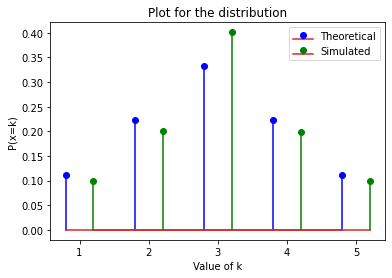
\includegraphics[scale=0.75]{plot.png}
\end{document}
